\documentclass[10pt, a4paper]{article}
\usepackage{fullpage}
\usepackage{graphicx}
\usepackage{subcaption}

\DeclareGraphicsExtensions{.jpg, .png}

\setlength{\parskip}{0.3cm}
\setlength{\parindent}{0cm}

\begin{document}
\title{Development Practice and Quality Assurance
\\ 3D Heap Visualisation}
\author{Aviv Beeri, Briony Goldsack, Ying Jiang, 
\\ Oliver Myerscough, Anna Thomas, Eleanor Vincent}
\maketitle

\section{Introduction}

An object-oriented software application creates complex structures on the heap during its lifetime. Debugging object-oriented software often involves thinking about how the heap evolves as a program runs. The aim of our group project is to design a tool which supports visualisation of the heap of a running Java program as a 3D scene which can be navigated by the software developer by moving around as if in a first person shooter game.

This report aims to present the methods we have employed to assure the quality of the software we are building and the techniques we have applied in our development process to ensure we deliver software smoothly and reliably. 

\section{Development Practices}

This section details the development practices we have chosen to employ, why we chose these techniques and our experience carrying them out. 

\subsection{Version Control}

Version control is a fundamental feature of any software project. The main benefits of version  control arise in the face of loss and reverting changes in the case of bugs.

We have chosen Git as our source control and back-up system over alternatives such as SVN, Mercurial and Bazaar for several reasons. Firstly, our previous experience of Git gives it an advantage and has allowed us to quickly and easily integrate it into the project. Git's branching model allows users to have multiple local branches that can be entirely independent of each other and the creation, merging and deletion of these branches is the fastest of the alternatives. This is ideal for group project work as it will enable us to experiment with different ideas without fear of breaking existing features and losing previous work. A crucial feature of Git is that it is distributed rather than centralised, unlike CVS and SVN. This means that when we are using a centralised workflow, every user has a full backup of the main server, each of which could be pushed up to replace the main server in the event of a crash or corruption. There is no single point of failure as multiple clones of the repository exist on multiple machines. Another major factor for choosing Git was the expansion to GitHub, which provided a friendly user-interface to work with. 

As we are using Git within our project it is important for us to use it effectively throughout all stages of our development. One way we do this is by having specific release branches on completion of key features. These are single commit branches that show the code at that particular state, ideally with no bugs in the code. This is a good process if we were doing weekly releases of the program because bug fixes could be pushed specifically to that branch and not become re-contaminated by new features that had begun since that release.

Alongside this members will often be working on certain elements of their tasks within their own branches before pushing to the master branch. This ensures that code does not inconsistently interrupt other people’s features and enables the team to keep the git logs clear and coherent throughout production. Having different merge commits of multiple branches full of chronological commits is much easier to use when working out the different states of the code than if different peoples commits kept overlapping within one common branch. The important thing to remember in doing this is that the period between each merge must not become too long as then we run the risk of the code base becoming too different from the branch version, making merging more complicated than the code itself, perhaps even taking more time than the project could afford.

\subsection{Automated Build Process}

An automated build process compiles the code and runs unit tests in one step, reducing manual processes. It is essential for building and testing our code quickly and reliably, ensuring that every member of the team is building the project in the same way. This improves the security and consistency of the code being written. 

Since we don’t all have the same setup for developing code, we chose to use a standard build system to compile the canonical version of our project and automate packaging it into a jar. We chose Gradle. We were put off build tools like Maven and Ant because they specify build scripts in XML, whereas Gradle lets us write our build scripts in Groovy DSL, a much more pleasant experience. This makes the build script much easier to comprehend compared to Maven. Maven does sport a powerful dependency management system with automated dependency fetching which would save us time. Rather than spend time searching for libraries group members can write code. This is a moot point as Gradle can be configured to hook into the Maven repositories, providing exactly the same functionality. Furthermore, Gradle is very flexible compared to Maven, allowing almost everything about a project to be configured. 

\subsection{Pair Programming}

Pair programming is a technique some consider quite integral to the extreme programming agile methodology and a number of organisations use it as part of their development practices. It works on the principle of a “driver” and a “navigator”, where the driver has the job of focusing on the current piece of coding required, while the navigator is charged with having a view towards the larger goal of completing the assigned task of the pair, worrying about the overall design and program structure. There is evidence which suggests that this produces a higher quality of code as it has been checked and discussed between two people, resulting in better design and readability, as well as fewer errors\textsuperscript{\cite{pairprog1a,pairprog1b,pairprog1c,pairprog1d}}.

It is important to note that there is the opinion that pair programming is not a universal method that is suitable everywhere. It depends heavily on the programmers involved. Some people have better habits and are predisposed to working together, but the more solitary worker would not be well suited to a pair programming environment\textsuperscript{\cite{partswap}}.

We have decided that our development practice will include the use of pair programming  which we hope will result in both an increase in the quality of code, as code will be sanity checked by multiple pairs of eyes, but also a better distribution of knowledge about our project across the entire team which is important because we have had past experiences where an individual becomes an “island of knowledge”, someone who is the only team member highly knowledgeable about particular key components of a system. This is something we want to avoid, so that they do not become essential for the further development of that area in the project\textsuperscript{\cite{pairprog2}}.

The way we will be trying to use pair programming is as follows:
At the start of each sprint, we will split into pairs to work on our tasks. At the very least, the task will begin with pair programming, so each team gets some understanding of the code relevant to the task at hand. At the beginning of the next sprint, we swap partners so that one person from a pair will work on a completely different area, the other on a similar one. In this way, knowledge can be passed between us on every part of the system, which is important, given the scale of the project.

\subsection{Continuous Integration}

One option of reducing the integration problems is continuous integration(CI)\textsuperscript{\cite{continuous1,continuous2}}. The main idea is to “eliminate blind spots so you can build and deliver software more rapidly”.  Every ‘push’ made by the team is checked by an automated build(i.e. Gradle), preventing the team work on an obviously broken repository. The CI server will notify the team about the build results depending on the behaviour of CI server. When a build fails, the team should not make any new commits until current problem is solved. This is particularly important when the team members work at different locations. The member who commits a ‘broken’ build should take responsibilities for solving the problem before going back home. 

Continuous integration has many advantages including fast for catching  issues and hence repairing, more time for adding features rather than debugging, easy for everyone in the team to get latest version and  low risks of each release. On the other hand, It is possible for ‘broken code’ to pass a test suite and get committed  due to the limitations of testing.

Our choice is Travis CI, a CI server that can be easily installed and integrated with GitHub.  Compared with Jenkins(another popular CI server), Travis is quick to get started and simple to have minimal configuration. It is also possible if users want to have more features. For instance, you can specify branches to build by whitelist or blacklist branches in .travis.yml. The result of builds are console output.

\section{Quality Assurance}

This sections addresses the processes we have in place to ensure our product is always in a good working condition and maintaining consistent quality throughout.

\subsection{Test-Driven Development (TDD)}

TDD combines test-first development and refactoring by writing an initial test case before writing and refactoring the code to pass it. Test-driven development is a key feature of extreme programming and has several advantages. Firstly, writing the tests first ensures that the developer focuses on fulfilling the requirements of the code. The unit tests can also be used as a detailed specification. Probably most importantly, TDD tells you immediately when your last change has broken previously working code. Furthermore, from a software design point of view, TDD helps create loosely coupled SOLID code. An argument against TDD is that it is hard to learn (a view of Mark Levison with which we sympathise\textsuperscript{\cite{mark}}) and can reduce productivity because of this, however, having practiced TDD previously we feel that this disadvantage is negated. 

Programming in Java, we are using JUnit to implement TDD. We picked JUnit because it is familiar and straightforward. Furthermore, JUnit can easily be integrated with Gradle using it’s Java plugin to create a quick and intuitive way to run tests using the ‘test’ task. Gradle will not build the project if there are failing tests unless the ‘test’ task is manually excluded. After running tests, Gradle produces HTML formatted reports which make it very easy to get both a general overview of the results and look at particular tests.

An example of our HTML Gradle report:

\begin{figure}[h]
	\centering
	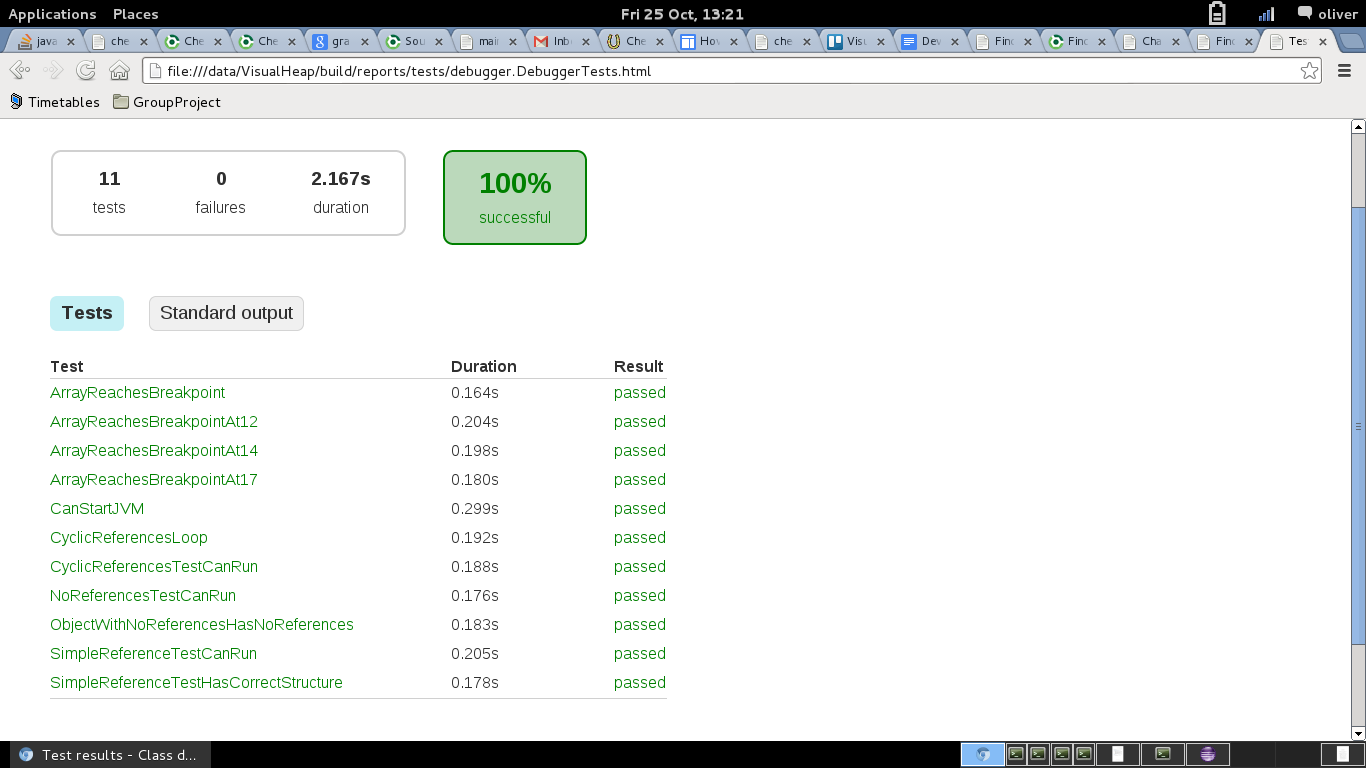
\includegraphics[width=\textwidth]{images/testresults.png}
	\caption{Running Tests with Gradle}
\end{figure}

\subsection{Coding Standards and documentation}

Coding standards define a programming style to be used throughout a software project. We have chosen to implement the following coding standards:
\begin{itemize}

  \item Naming conventions
  \item File naming and organisation
  \item Formatting and indentation
  \item Comments and Documentation
  \item Testing

\end{itemize}
It can be summarised that the main benefits of maintaining a coding standard are readability, maintainability and compatibility. It is particularly important regarding pair programming and swapping partners as any member of the team should be able to read the code of any other member. On the other hand, several arguments against coding standards have been identified, as discussed by Zac Gery\textsuperscript{\cite{zac}}. Such disadvantages that we agree should be highlighted are that standards such as spacing and comments could be seen as micro-managing and each new rule adds to the complexity of the implementation and could distract from the larger goal of building, testing and releasing functionality to a deadline. With these criticisms of coding standards in mind we have decided to keep our guidelines sensible, intuitive and minimal. An alternative approach could be to use code reviews, which can help developers focus on larger concerns such as architectural issues, prompt discussions and permit suggestions. However, code reviews can be time consuming. We feel that a joint approach would be most beneficial, whereby we have a set of coding standards and also perform intermittent code reviews within our pair programming groups. Code documentation is important when working in a group as it provides a convenient way of of understanding the code written by others. We have decided to employ Javadoc to generate code documentation as it is easy to keep up to date as the documentation is within the program itself.

\section{Supervisor Discussion}

The feedback from our supervisor regarding our development practices and quality assurance methods was particularly useful in defining our implementation process. We were encouraged to think about the range of version control tools and automated build processes available and those most suited to our project. We also researched the use of these techniques in industry, in particular, pair programming, and how methods such as test-driven development and continuous integration fit within agile development. Our supervisor also highlighted the importance of coding standards and code documentation to improve code clarity and quality. From this discussion with our supervisor, we improved our development practices by implementing a set of coding standards and ensuring that we followed a continuous integration culture, understanding its importance in extreme programming. 

\section{Conclusion}

The development practices we have chosen to implement such as  continuous integration (CI) and test-driven development (TDD) integrate well with the iterations of agile development to provide high quality code and project flexibility. A CI culture ensures the efficient development of quality software, while TDD provides quick feedback. The Gradle automated build process further supports continuous integration by running tests to detect integration errors as quickly as possible. In addition, the use of version control using Git underpins CI culture by encouraging commits to be made little and often.

\begin{thebibliography}{9}

\bibitem{partswap}
  Tim Ottinger, Jeff Langr,
  \emph{Partner swapping},
  \\http://agileinaflash.blogspot.co.uk/2009/02/pair-programming-smells.html

\bibitem{glen}
  Glen Stansberry,
  \emph{7 Version Control Systems Reviewed},
  \\http://www.smashingmagazine.com/2008/09/18/the-top-7-open-source-version-control-systems/
  
\bibitem{mark}
  Mark Levison,
  \emph{Advantages of TDD},
  \\http://agilepainrelief.com/notesfromatooluser/2008/10/advantages-of-tdd.html
  
\bibitem{zac}
  Zac Gery,
  \emph{Coding Standards Are Overrated},
  \\http://java.dzone.com/articles/coding-standards-are-overrated

\bibitem{continuous1}
  ThoughtWorks, Inc.,
  \emph{Continuous Integration},
  \\http://www.thoughtworks.com/continuous-integration

\bibitem{continuous2}
  Mark van Lent,
  \emph{Continuous Integration},
  \\http://www.vlent.nl/weblog/2012/10/12/travis-ci-easy-and-fun-ci-for-your-plone-packages-nejc-zupan/ 

\bibitem{pairprog1a}
  Don Wells,
  \emph{Pair Programming},
  \\http://www.extremeprogramming.org/rules/pair.html
  
\bibitem{pairprog1b}
  Agile Alliance, Institut Agile.,
  \emph{Pair Programming},
  \\http://guide.agilealliance.org/guide/pairing.html
  
\bibitem{pairprog1c}
  John Griffin,
  \emph{Pair Programming},
  \\http://www.johng.co.uk/2010/07/04/pair-programming-pros-and-cons/

\bibitem{pairprog1d}
  Jon Evans,
  \emph{Pair Programming},
  \\http://techcrunch.com/2012/03/03/pair-programming-considered-harmful/ 

\bibitem{pairprog2}
  VersionOne, Inc.,
  \emph{Pair Programming},
  \\http://www.versionone.com/Agile101/Pair{\_}Programming.asp

\end{thebibliography}

\end{document}
